\documentclass[tikz]{standalone}
\usetikzlibrary{shapes.geometric}
\begin{document}%
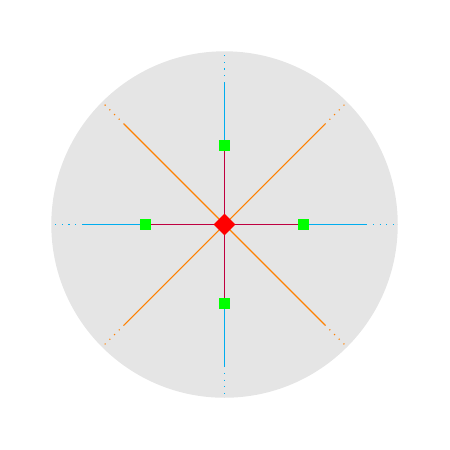
\begin{tikzpicture}
\useasboundingbox (0,0) circle (2.5cm);

\fill[gray!20] (0,0) circle (2.2cm);

\coordinate (C) at (0,0);
\coordinate (B0) at (1,0);
\coordinate (B1) at (0,1);
\coordinate (B2) at (-1,0);
\coordinate (B3) at (0,-1);

\draw[purple] (C) -- (B0);
\draw[purple] (C) -- (B1);
\draw[purple] (C) -- (B2);
\draw[purple] (C) -- (B3);

\draw[cyan] (B0) -- (1.8,0);
\draw[cyan,dotted] (1.8,0) -- (2.2,0);
\draw[cyan] (B1) -- (0,1.8);
\draw[cyan,dotted] (0,1.8) -- (0,2.2);
\draw[cyan] (B2) -- (-1.8,0);
\draw[cyan,dotted] (-1.8,0) -- (-2.2,0);
\draw[cyan] (B3) -- (0,-1.8);
\draw[cyan,dotted] (0,-1.8) -- (0,-2.2);

\draw[orange] (C) -- (45:1.8cm);
\draw[orange,dotted] (45:1.8cm) -- (45:2.2cm);
\draw[orange] (C) -- (135:1.8cm);
\draw[orange,dotted] (135:1.8cm) -- (135:2.2cm);
\draw[orange] (C) -- (225:1.8cm);
\draw[orange,dotted] (225:1.8cm) -- (225:2.2cm);
\draw[orange] (C) -- (315:1.8cm);
\draw[orange,dotted] (315:1.8cm) -- (315:2.2cm);

\node[diamond,fill=red,inner sep=2pt] at (C) {};

\foreach \x in {0,1,...,3}
\node[rectangle,fill=green,inner sep=2pt] at (B\x) {};

\end{tikzpicture}%
\end{document}
